% \documentclass[handout]{beamer}
\documentclass{beamer}

\mode<presentation>
{
  \usetheme{default}
  \usefonttheme[onlymath]{serif}
  % \usetheme{Singapore}
  % \usetheme{Warsaw}
  % \usetheme{Malmoe}
  % \useinnertheme{circles}
  % \useoutertheme{infolines}
  % \useinnertheme{rounded}
  %\setbeamercovered{transparent=100}
}

\usepackage[english]{babel}
\usepackage[latin1]{inputenc}
\usepackage{alltt,listings,multirow,ulem,siunitx}
\usepackage[absolute,overlay]{textpos}
\TPGrid{1}{1}
\usepackage{pdfpages}
\usepackage{multimedia}
\newcommand\hmmax{0}
\newcommand\bmmax{0}
\usepackage{bm}

% font definitions, try \usepackage{ae} instead of the following
% three lines if you don't like this look
\usepackage{mathptmx}
\usepackage[scaled=.90]{helvet}
% \usepackage{courier}
\usepackage[T1]{fontenc}
\usepackage{tikz}
\usetikzlibrary[shapes,shapes.arrows,arrows,shapes.misc,fit,positioning,trees,mindmap,backgrounds]

% \usepackage{pgfpages}
% \pgfpagesuselayout{4 on 1}[a4paper,landscape,border shrink=5mm]

\usepackage{JedMacros}

\title{High Performance Implicit Solvers for Geodynamics}
\subtitle{These slides: \url{http://59A2.org/files/20130110-CIGWebinar.pdf}}
\author{{\bf Jed Brown} \\ \url{jedbrown@mcs.anl.gov}}

% - Use the \inst command only if there are several affiliations.
% - Keep it simple, no one is interested in your street address.
\institute
{
  {Mathematics and Computer Science Division, Argonne National Laboratory} \\
}

\date{CIG Webinar 2013-01-10}

% This is only inserted into the PDF information catalog. Can be left
% out.
\subject{Talks}


% If you have a file called "university-logo-filename.xxx", where xxx
% is a graphic format that can be processed by latex or pdflatex,
% resp., then you can add a logo as follows:

% \pgfdeclareimage[height=0.5cm]{university-logo}{university-logo-filename}
% \logo{\pgfuseimage{university-logo}}



% Delete this, if you do not want the table of contents to pop up at
% the beginning of each subsection:
% \AtBeginSubsection[]
% {
% \begin{frame}<beamer>
%   \frametitle{Outline}
%   \tableofcontents[currentsection,currentsubsection]
% \end{frame}
% }

\AtBeginSection[]
{
  \begin{frame}<beamer>
    \frametitle{Outline}
    \tableofcontents[currentsection]
  \end{frame}
}

% If you wish to uncover everything in a step-wise fashion, uncomment
% the following command:

% \beamerdefaultoverlayspecification{<+->}

\begin{document}
\lstset{language=C}
\normalem

\begin{frame}
  \titlepage
\end{frame}

\begin{frame}{Outline}
  \tableofcontents
\end{frame}

\section{Role of implicit solvers}
\begin{frame}{Why do we need solvers?}
  \begin{definition}[Stiffness]
    A discretized PDE is stiff if the true physics propagates information much more than one grid cell over a time step length desirable for resolving transient dynamics.
  \end{definition}
  \vspace{-1.5em}
  \uncover<2->{
  \begin{gather*}
    {\color<5->{gray} (\rho\uu)_t} + \div ({\color<4->{gray} \rho\uu\otimes\uu} - \eta D\uu + p\bm 1) - \rho \bm g = 0 \\
    {\color<3->{gray} \rho_t} + \div \rho\uu = 0
  \end{gather*}}
  \vspace{-1.5em}
  \begin{enumerate}
  \item<3-> Incompressibility: acoustic wave travels much faster than mantle or lithosphere time scale (anelastic; Mach number)
  \item<4-> Convection insignificant compared to viscosity (unrelated to stiffness; Reynolds number)
  \item<5-> Relaxation fast compared to dynamical time scale (depends on observational scale)
  \end{enumerate}
\end{frame}
\begin{frame}
  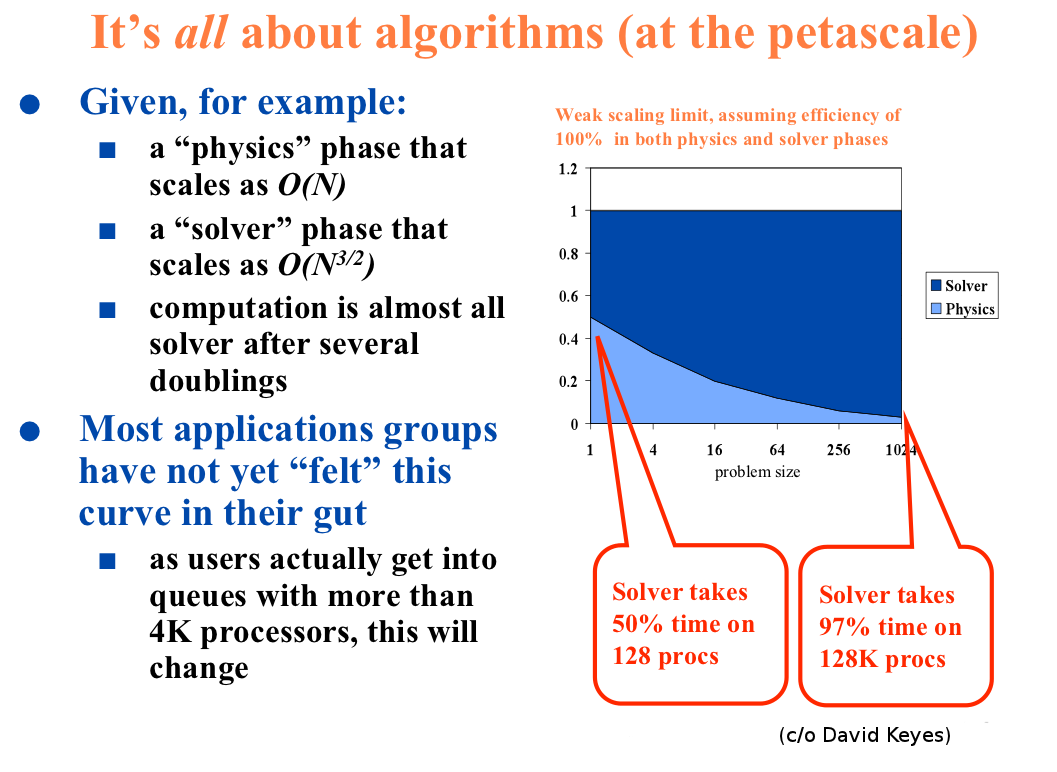
\includegraphics[width=1.05\textwidth]{figures/KeyesAllAboutAlgorithms}
\end{frame}

\section{Common methods and algorithmic barriers}
\begin{frame}{Evaluating methods}
  \begin{itemize}
  \item Performance of methods will depend on \alert{grid resolution} and \alert{model parameters} (regime and heterogeneity).
  \item A method is:
    \begin{itemize}
    \item \alert{scalable} (also ``optimal'') if its performance is independent of resolution and parallelism
    \item \alert{robust} if its performance is (nearly) independent of model parameters
    \item \alert{efficient} if it solves the problem in a small multiple of the cost to evaluate the residual\footnote{We'll settle for ``as fast as the best known method''.}
    \end{itemize}
  \item<2-> Linear problems typically arise from linearizing a nonlinear problem.
    This step is \alert{not necessary}, but it is convenient for \alert{reusing software} and for \alert{debugging}.
  \end{itemize}
\end{frame}
\begin{frame}{Taxonomy of implicit solvers}
  \begin{block}{Global linearization: Picard and Newton}
    \begin{itemize}
    \item Linear solve ``$J(u) w = -F(u)$''
      \begin{itemize}
      \item (sparse) direct vs. iterative (Krylov) with preconditioning
      \item classical relaxation (Jacobi, Gauss-Seidel), incomplete factorization (ILU)
      \item \alert<2->{domain decomposition and multigrid}
      \end{itemize}
    \item Globalization: ``$u_{\text{next}} = u + \alpha w$''
      \begin{itemize}
      \item Line search, trust region, continuation
      \end{itemize}
    \end{itemize}
  \end{block}
  \begin{block}{Inherently nonlinear methods}
    \begin{itemize}
    \item Nonlinear GMRES, Nonlinear CG (can use preconditioning)
    \item \alert<2->{Nonlinear domain decomposition}
    \item \alert<2->{Nonlinear multigrid: Full Approximation Scheme (FAS)}
    \end{itemize}
  \end{block}
  \begin{itemize}
  \item<2-> \only<2>{\alert{These methods can be {\bf scalable}.}}
    \only<3>{\alert{How nonlinear are the scales? How expensive is setup?}}
  \end{itemize}
\end{frame}

\begin{frame}{What about direct linear solvers?}
  \begin{centering}
    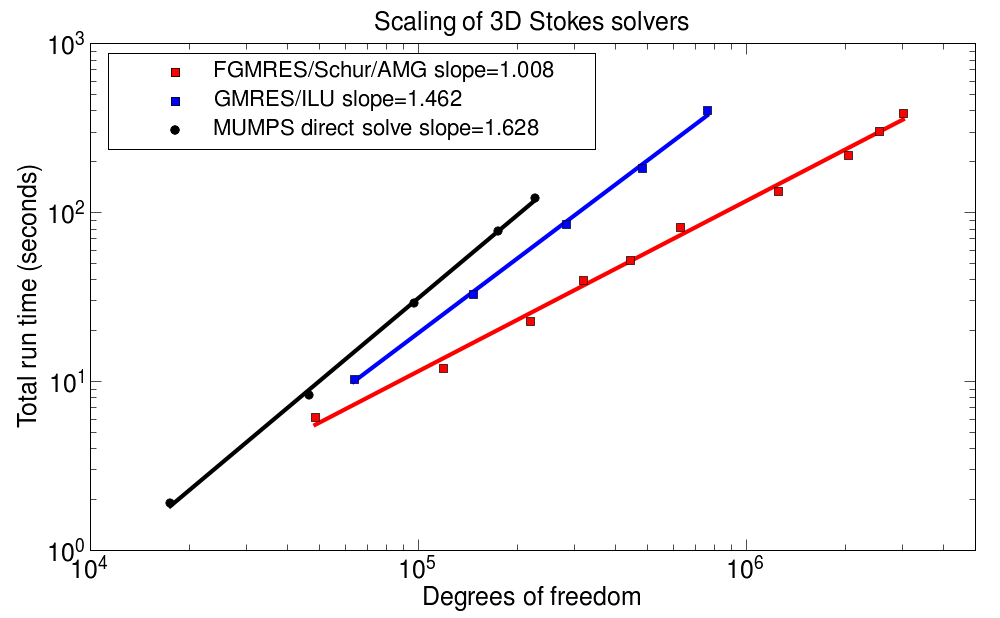
\includegraphics[width=0.8\textwidth]{figures/MG/StokesScalingDirectVsChebySchur}
  \end{centering}
  \begin{itemize}
  \item By all means, start with a direct solver
  \item Direct solvers are \alert{robust}, but \alert{not scalable}
  \item {\bf 2D}: $\bigO(n^{1.5})$ flops, $\bigO(n\log n)$ memory.
  \item {\bf 3D}: $\bigO(n^2)$ flops, $\bigO(n^{4/3})$ memory
  \item We will focus on \alert{iterative} linear solvers
  \end{itemize}
\end{frame}
\begin{frame}{Matrices}
  \begin{definition}<1->[Matrix]
    A \alert{matrix} is a linear transformation between finite dimensional vector spaces.
  \end{definition}
  \begin{definition}<2->[Forming a matrix]
    \alert{Forming} or \alert{assembling} a matrix means defining it's action in terms of entries (usually stored in a sparse format).
  \end{definition}
\end{frame}

\begin{frame}{Important matrices}
  \begin{enumerate}
  \item Sparse (e.g.~discretization of a PDE operator)
  \item \alert<2,4>{Inverse of \emph{anything} interesting $B = A^{-1}$}
  \item \alert<4>{Jacobian of a nonlinear function $J y = \lim_{\epsilon \to 0} \frac{F(x + \epsilon y) - F(x)}{\epsilon}$}
  \item \alert<2,4>{Fourier transform $\mathcal{F},\mathcal{F}^{-1}$}
  \item \alert<2,4>{Other fast transforms, e.g. Fast Multipole Method}
  \item \alert<2,4>{Low rank correction $B = A + u v^T$}
  \item \alert<2,4>{Schur complement $S = D - C A^{-1} B$}
  \item \alert<3,4>{Tensor product $A = \sum_e A_x^e \otimes A_y^e \otimes A_z^e$}
  \item \alert<3,4>{Linearization of a few steps of an explicit integrator}
  \end{enumerate}
  \begin{columns}\begin{column}{0.3\textwidth}\end{column}\begin{column}{0.7\textwidth}
  \begin{itemize}
  \item<only@2> These matrices are \alert<2>{dense}.  Never form them.
  \item<only@3>{Thes are \alert<3>{not very sparse}.}
    Don't form them.
  \item<only@4> {None of these matrices ``have entries''}
  \end{itemize}
\end{column}
\end{columns}
\end{frame}

\begin{frame}{What can we do with a matrix that doesn't have entries?}
  \begin{block}{Krylov solvers for $A x = b$}
    \begin{itemize}
    \item Krylov subspace: $\{b, Ab, A^2b, A^3b, \dotsc\}$
    \item Convergence rate depends on the spectral properties of the matrix
      \begin{itemize}
      \item Existance of small polynomials $p_n(A) < \epsilon$ where $p_n(0) = 1$.
      \item condition number $\kappa(A) = \norm{A} \norm{A^{-1}} = \sigma_{\text{max}}/\sigma_{\text{min}}$
      \item distribution of singular values, spectrum $\Lambda$, pseudospectrum $\Lambda_\epsilon$
%      \item $\epsilon$-pseudospectrum $\Lambda_\epsilon$, spectrum of $A + E$ where $\norm{E} < \epsilon$
      \end{itemize}
    \item For any popular Krylov method $\mathcal{K}$, there is a matrix
      of size $m$, such that $\mathcal{K}$ outperforms all other methods
      by a factor at least $\bigO(\sqrt{m})$~[Nachtigal et. al., 1992]%\cite{nachtigal1992fnm}
    \end{itemize}
  \end{block}
  \begin{block}{Typically...}
    \begin{itemize}
    \item The action $y \gets A x$ can be computed in $\bigO(m)$
    \item Aside from matrix multiply, the $n^{\text{th}}$ iteration requires at most $\bigO(mn)$
    \end{itemize}
  \end{block}
\end{frame}

\begin{frame}{The $\pfrak$-Bratu equation}
  \begin{itemize}
  \item 2-dimensional model problem
    \begin{equation*}
      -\div \big(\abs{\nabla u}^{\pfrak-2} \nabla u \big) - \lambda e^u - f = 0, \qquad 1 \le \pfrak \le \infty, \quad \lambda < \lambda_{\text{crit}}(\pfrak)
    \end{equation*}
    Singular or degenerate when $\nabla u = 0$, turning point at $\lambda_{\text{crit}}$.
  \item Regularized variant
    \begin{gather*}
      -\div (\alert<1>{\eta} \nabla u) - \lambda e^u - f = 0 \\
      \eta(\gamma) = (\epsilon^2 + \gamma)^{\frac{\pfrak-2}{2}} \qquad \gamma(u) = \half \abs{\nabla u}^2
    \end{gather*}
  \item Jacobian
    \begin{gather*}
      J(u) w \sim -\div \big[ \alert<1>{(\eta \bm 1 + \eta' \nabla u \otimes \nabla u)} \nabla w \big] - \lambda e^u w \\
      \eta' = \frac{\pfrak-2}{2} \eta / (\epsilon^2 + \gamma)
    \end{gather*}
    Interpretation: conductivity tensor flattened in direction $\nabla u$ %($\pfrak < 2$)
  \item Simple finite difference discretization in PETSc: \\
    \shell{cd petsc/src/snes/examples/tutorials/; make ex15}
  \item<2> \alert{Step 1: Write the residual.}
  \end{itemize}
\end{frame}
\begin{frame}{Step 1: Write the residual}
  \begin{itemize}
  \item Start with $\pfrak=2$ (standard Laplacian), define only residuals
  \item Matrix-free Jacobians, no preconditioning \code{-snes\_mf}
  \item \shell{./ex15 -da\_refine \alert{1} -snes\_mf -snes\_monitor -ksp\_converged\_reason}
    \only<2>{{\tiny \color{green!30!black} \tt \\
  0 SNES Function norm 9.324361041196e-01 \\
  Linear solve converged due to CONVERGED\_RTOL iterations 7\\
  1 SNES Function norm 4.534365556764e-09 \\
CONVERGED\_FNORM\_RELATIVE Number of nonlinear iterations = 1
}}
  \item \shell{./pbratu -da\_refine \alert{2} -snes\_mf -snes\_monitor -ksp\_converged\_reason}
    \only<3>{{\tiny \color{green!30!black} \tt \\
  0 SNES Function norm 5.363535697720e-01 \\
  Linear solve converged due to CONVERGED\_RTOL iterations 18\\
  1 SNES Function norm 1.276738526722e-06 \\
  Linear solve converged due to CONVERGED\_RTOL iterations 18\\
  2 SNES Function norm 1.263046904535e-11 \\
CONVERGED\_FNORM\_RELATIVE Number of nonlinear iterations = 2
}}
  \item \shell{./pbratu -da\_refine \alert{3} -snes\_mf -snes\_monitor -ksp\_converged\_reason}
    \only<4>{{\tiny \color{green!30!black} \tt \\
  0 SNES Function norm 2.820917170607e-01 \\
  Linear solve converged due to CONVERGED\_RTOL iterations 42\\
  1 SNES Function norm 2.782839451653e-06 \\
  Linear solve converged due to CONVERGED\_RTOL iterations 45\\
  2 SNES Function norm 2.682642095006e-11 \\
CONVERGED\_FNORM\_RELATIVE Number of nonlinear iterations = 2
}}
  \item \shell{./pbratu -da\_refine \alert{4} -snes\_mf -snes\_monitor -ksp\_converged\_reason}
    \only<5->{{\tiny \color{green!30!black} \tt \\
  0 SNES Function norm 1.441189193029e-01 \\
  Linear solve converged due to CONVERGED\_RTOL iterations 101\\
  1 SNES Function norm 1.409860069506e-06 \\
  Linear solve converged due to CONVERGED\_RTOL iterations 154\\
  2 SNES Function norm 1.390912345257e-11 \\
CONVERGED\_FNORM\_RELATIVE Number of nonlinear iterations = 2
}}
  \item<6> The number of iterations is growing with grid refinement.
  \end{itemize}
\end{frame}
\begin{frame}[fragile]{Experimenting with algorithms}
  \begin{itemize}
  \item \verb|-pc_type asm -sub_pc_type lu|
  \item \verb|-pc_type gamg -pc_gamg_agg_nsmooths 1|
  \item \verb|-jtype PICARD -pc_type lu|
  \item \verb|-snes_mf_operator -jtype PICARD -pc_type ml|
  \item \verb|-snes_type ngmres -snes_ngmres_m 10| \\
    \qquad \verb|-npc_snes_max_it 1 -npc_snes_type fas|
  \end{itemize}
\end{frame}

\begin{frame}[fragile]{Barriers}
  \begin{itemize}
  \item Krylov method: $(\text{iteration count}) \sim \sqrt{\text{condition number}}$
  \item Elliptic ill-conditioning
    \begin{itemize}
    \item $\kappa(A) \sim h^{-2}$ for second order elliptic problems
    \item \emph{Asymptotics} not improved for standard methods:\\
      \verb|-pc_type jacobi|, \verb|-pc_type sor|, \verb|-pc_type ilu|
    \item 1-level Domain Decomposition: $\kappa \sim H^{-2} \phi(H/h)$ \\
      \verb|-pc_type bjacobi|, \verb|-pc_type asm|
    \item Multilevel/multigrid: $\kappa \sim 1$ \\
      \verb|-pc_type gamg|, \verb|-pc_type ml|, \verb|-pc_type hypre|, \verb|-pc_type mg|
    \end{itemize}
  \item Heterogeneity
    \begin{itemize}
    \item Conditioning proportional to maximum material contrast
    \item In friendly circumstances, a local preconditioner restores $\sim h^{-2}$ ill-conditioning
    \item Coarse approximations and subdomain transmission conditions become difficult
    \item Fine grids necessary \emph{because of} heterogeneity
    \item Coarse grid must accurately represent long-range coupling
    \end{itemize}
  \end{itemize}
\end{frame}

\section{Failure modes and troubleshooting}
\begin{frame}{Low energy modes of preconditioned operator $P^{-1}A$}
  \framesubtitle{$2\times 2$ checkerboard elasticity problem, Neumann condition on right boundary}
  \vspace{-1em}
  \begin{itemize}
  \item {\scriptsize
    \only<1>{Original operator, stiff blocks don't move}
    \only<2>{With Jacobi preconditioning, balances stiffness, not $\bigO(\Delta x^2)$ elliptic ill-conditioning}
    \only<3>{With BoomerAMG preconditioning, does not find all rotations}
    \only<4>{With geometric MG, Galerkin coarse operators, Chebychev smoother}
    \only<5>{With geometric MG, Galerkin coarse operators, \alert{unstable} Chebychev smoother}
  }
  \end{itemize}
    \only<1>{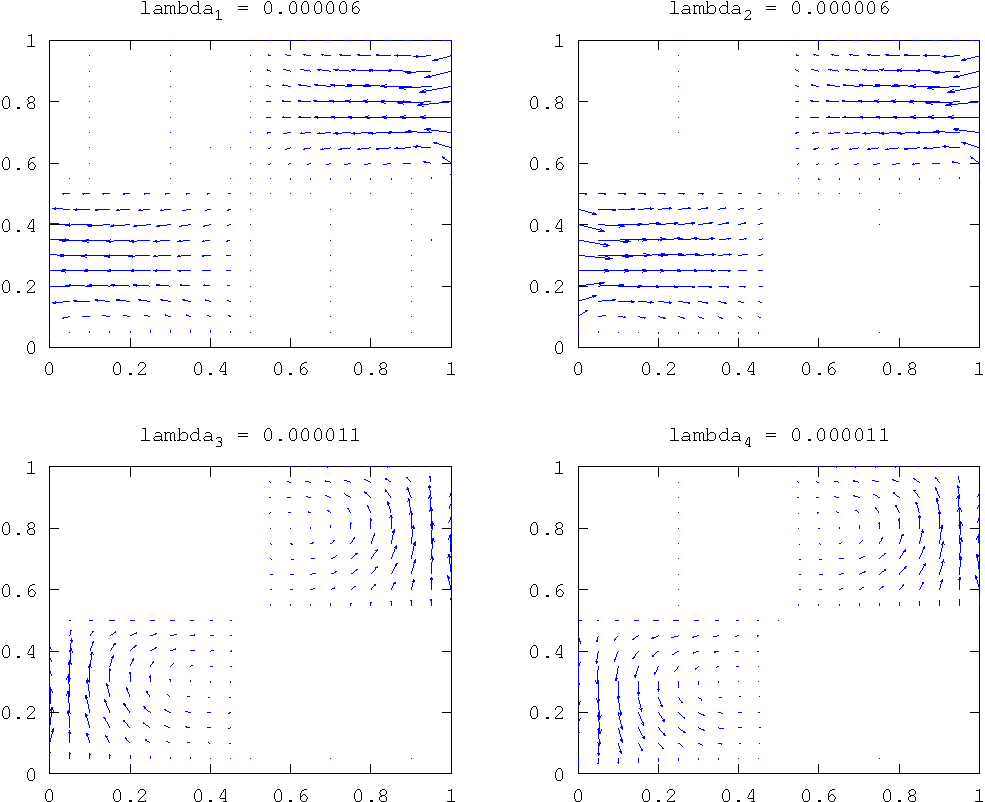
\includegraphics[width=0.7\textwidth]{figures/MG/ElastModesNone.pdf}}
    \only<2>{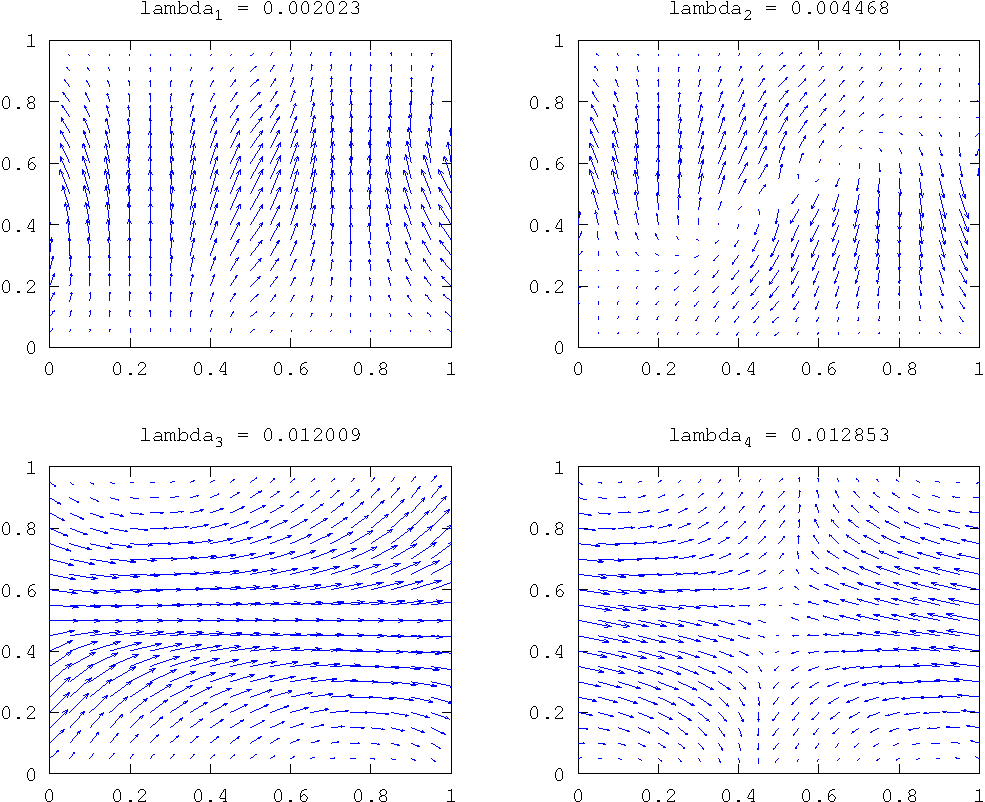
\includegraphics[width=0.7\textwidth]{figures/MG/ElastModesJacobi.pdf}}
    \only<3>{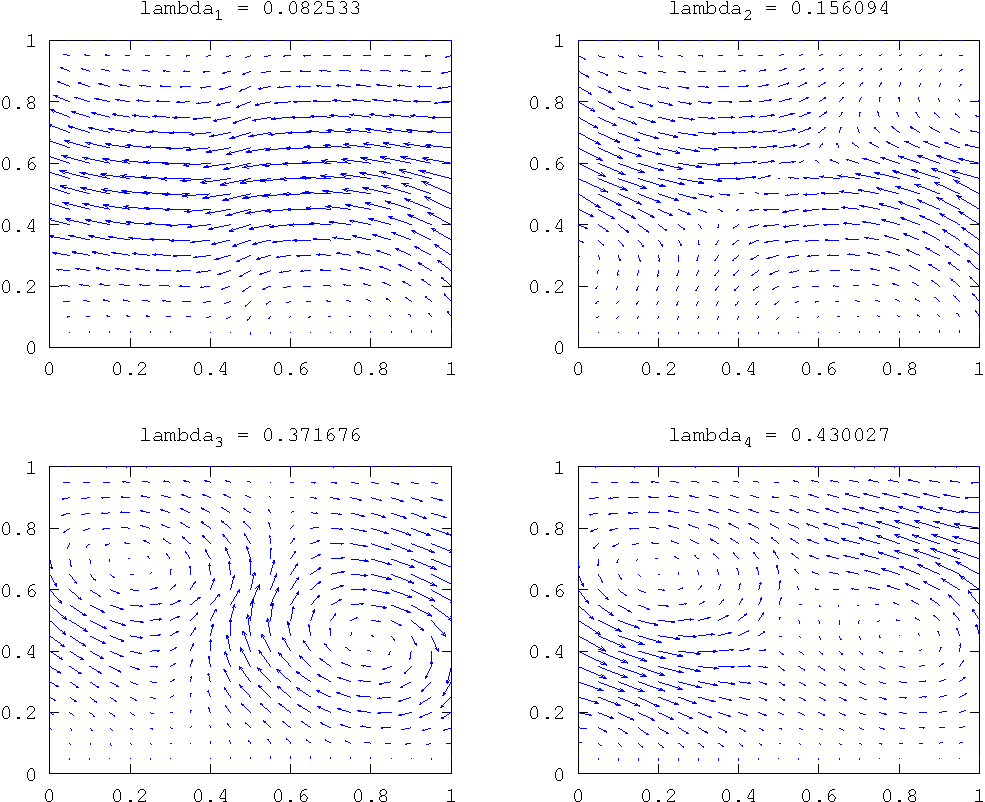
\includegraphics[width=0.7\textwidth]{figures/MG/ElastModesHypre.pdf}}
    \only<4>{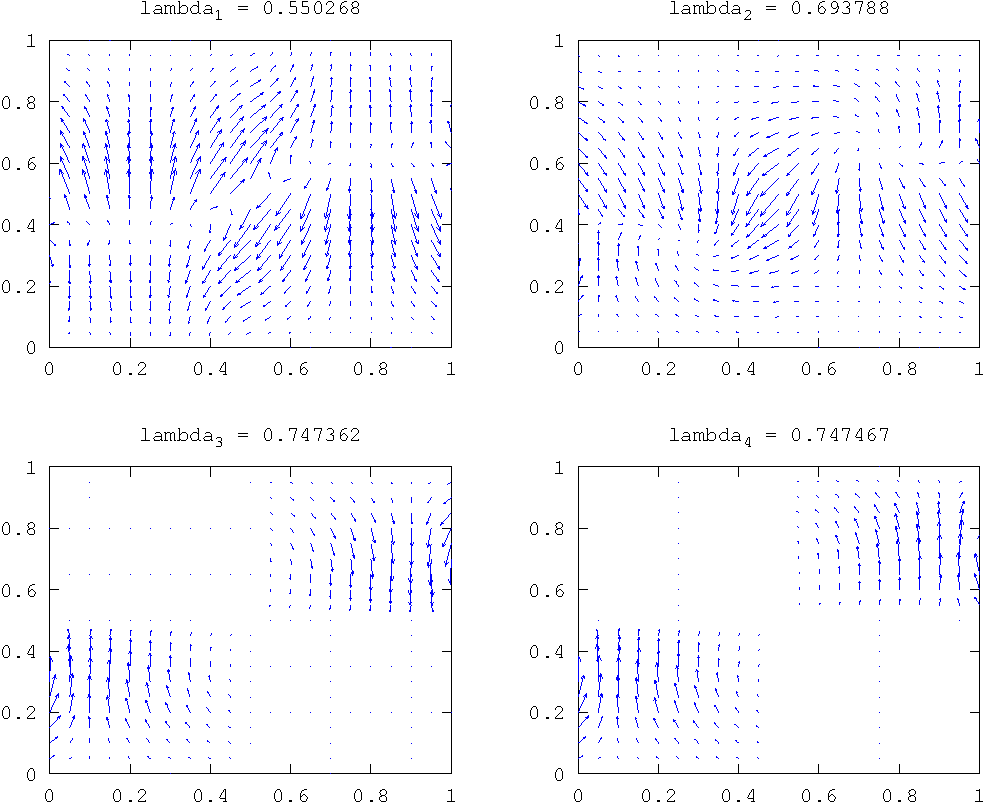
\includegraphics[width=0.7\textwidth]{figures/MG/ElastModesGMGGalerkin.pdf}}
    \only<5>{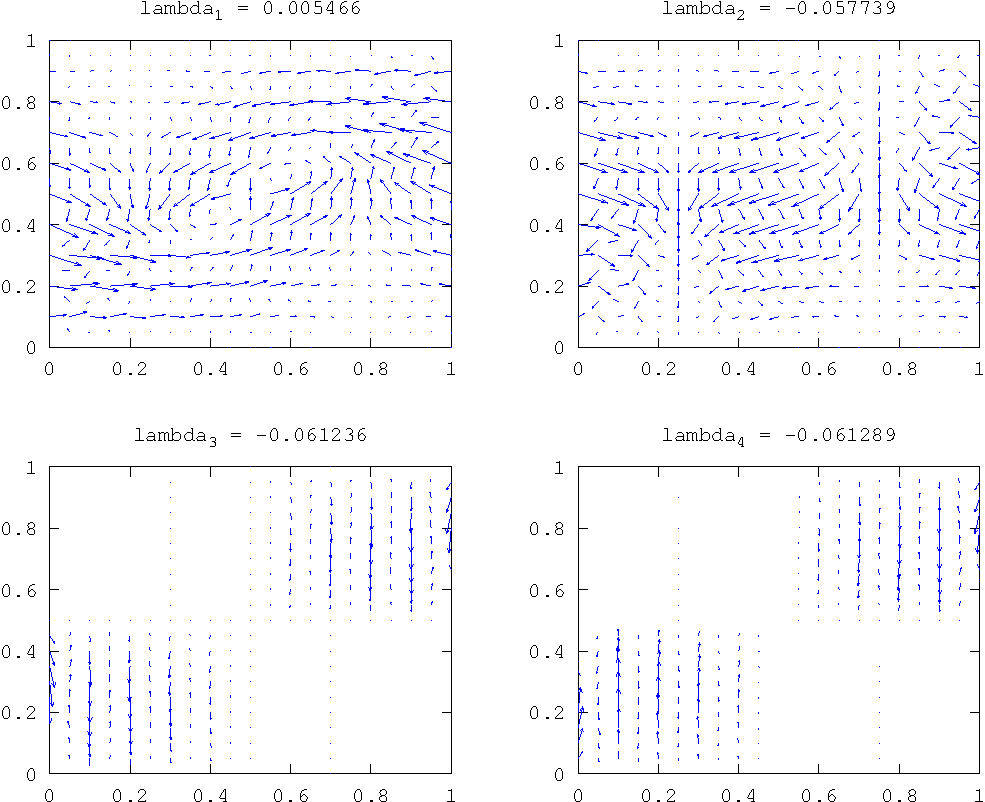
\includegraphics[width=0.7\textwidth]{figures/MG/ElastModesGMGGalerkinCheb2Unstable.pdf}}
    \begin{textblock}{0.3}[1,0.5](1,0.5)
      \only<1>{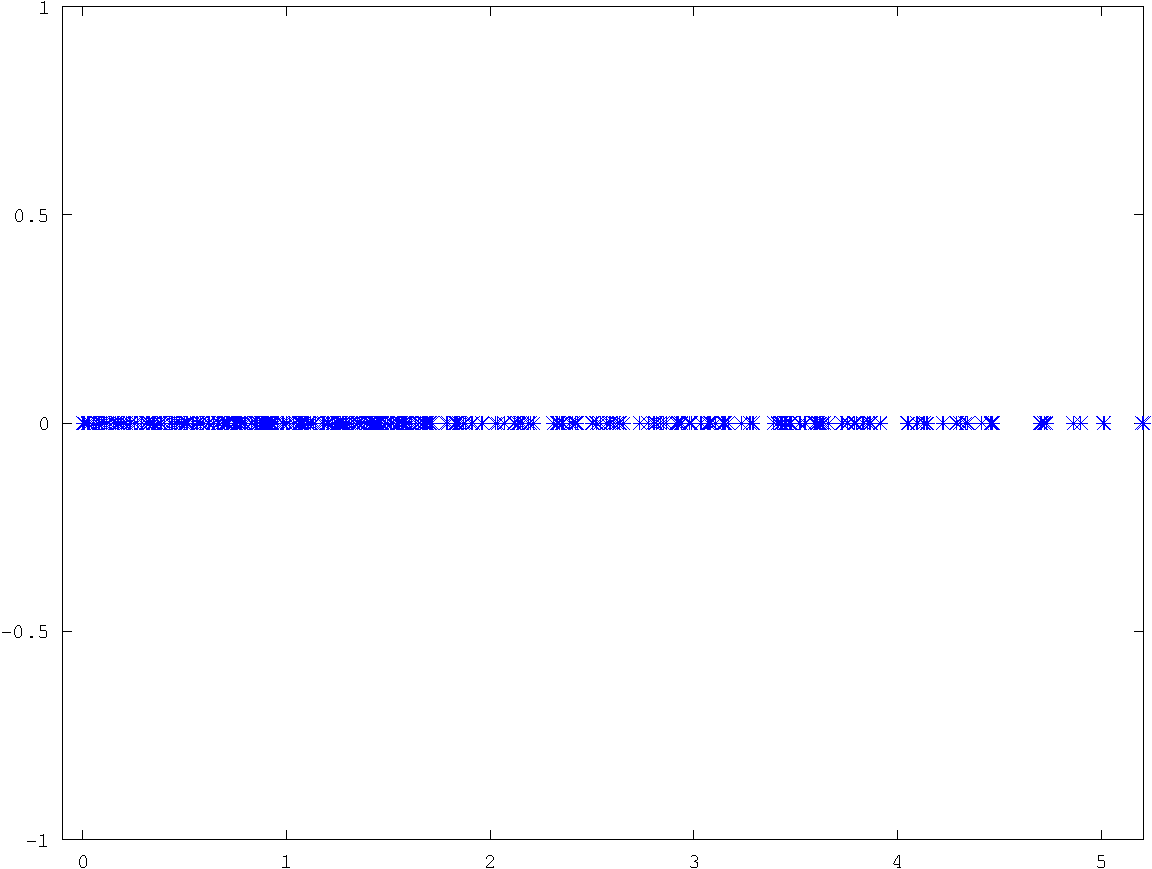
\includegraphics[width=\textwidth]{figures/MG/ElastEigsNone.pdf}}
      \only<2>{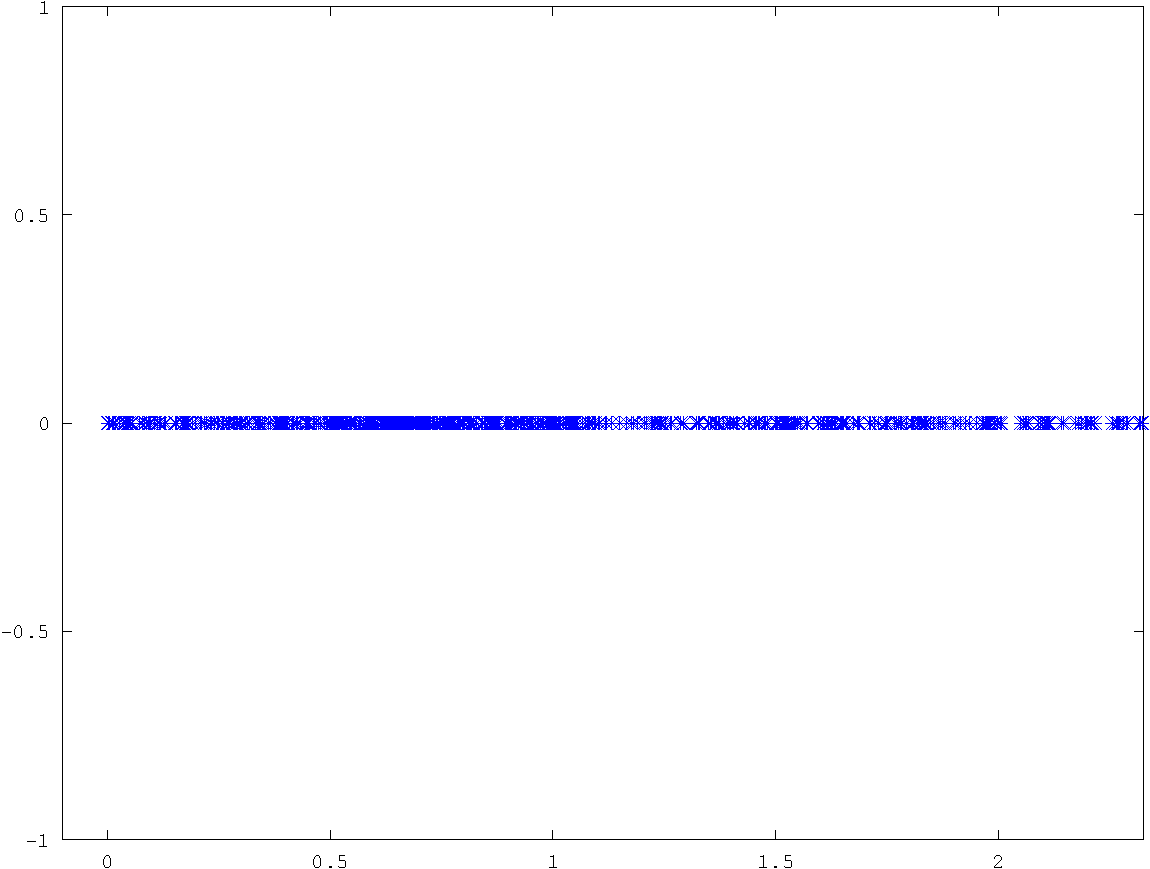
\includegraphics[width=\textwidth]{figures/MG/ElastEigsJacobi.pdf}}
      \only<3>{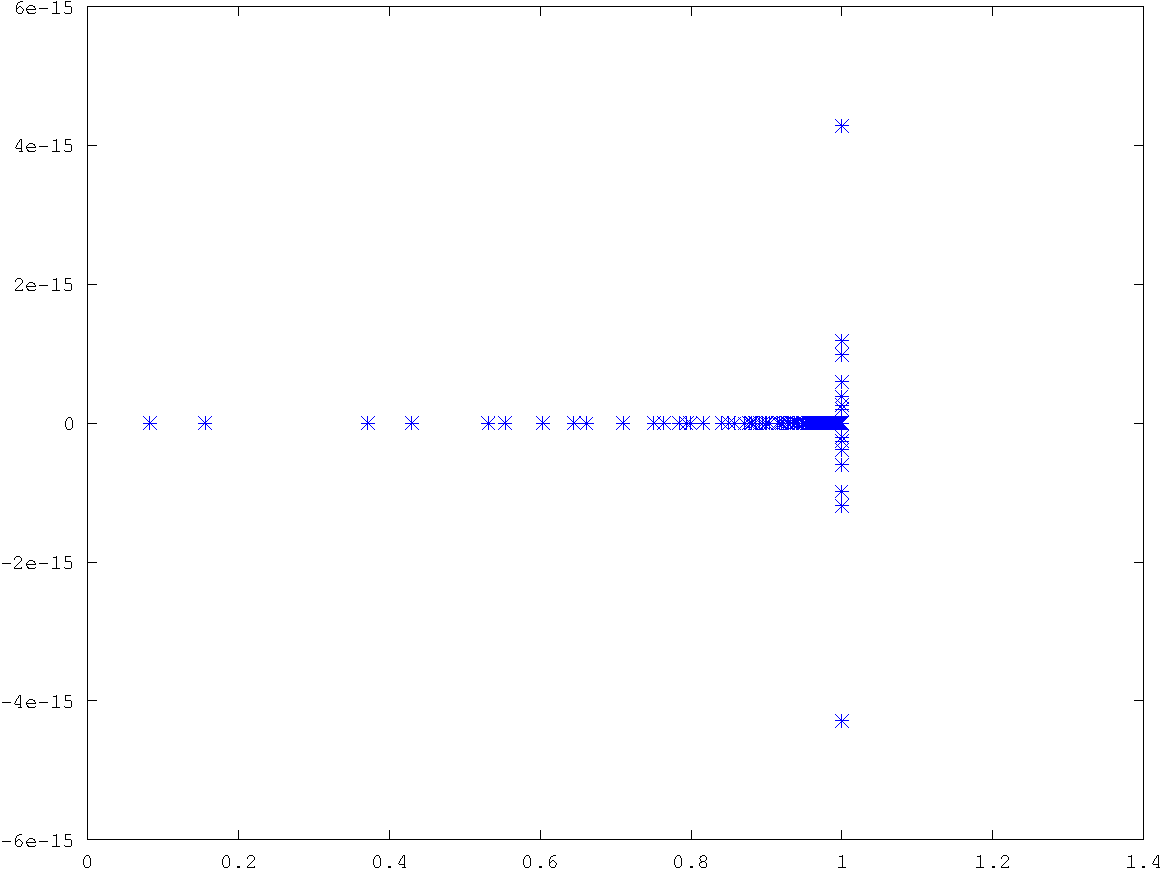
\includegraphics[width=\textwidth]{figures/MG/ElastEigsHypre.pdf}}
      \only<4>{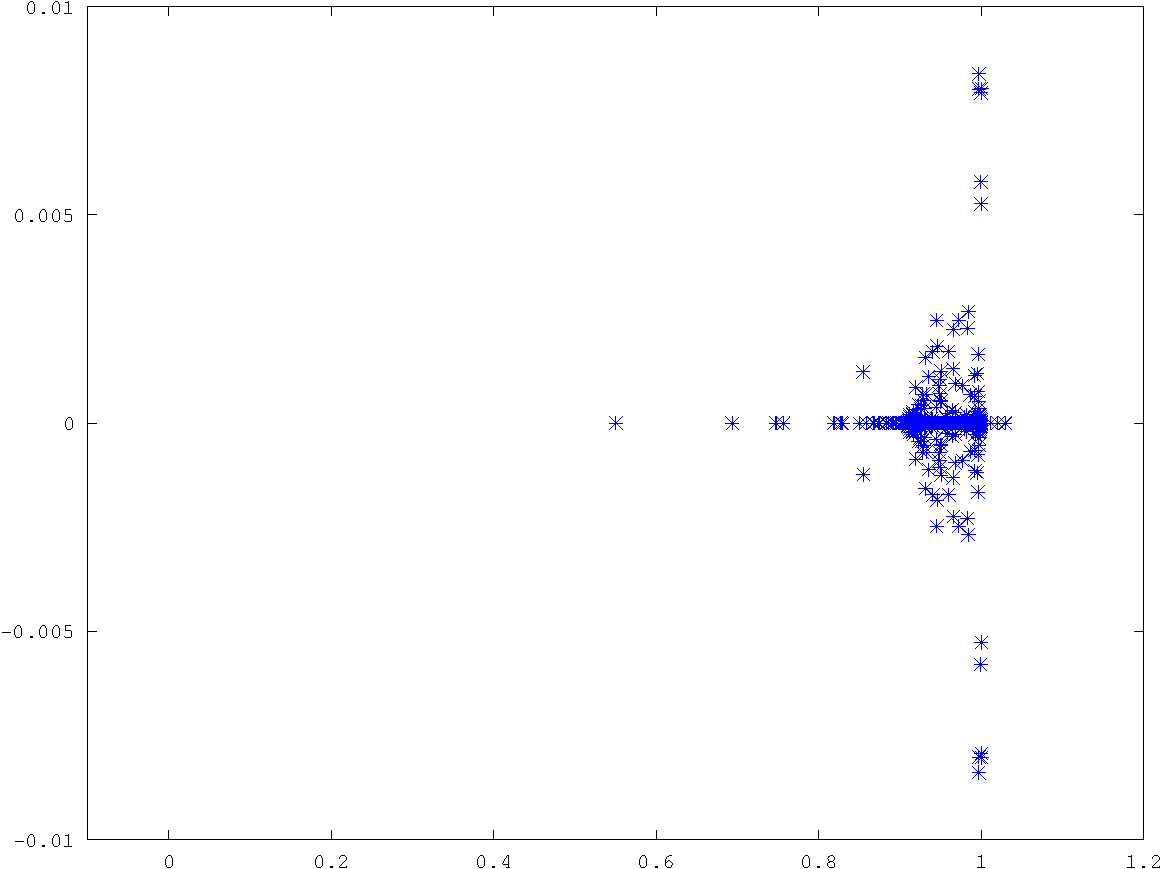
\includegraphics[width=\textwidth]{figures/MG/ElastEigsGMGGalerkin.pdf}}
      \only<5>{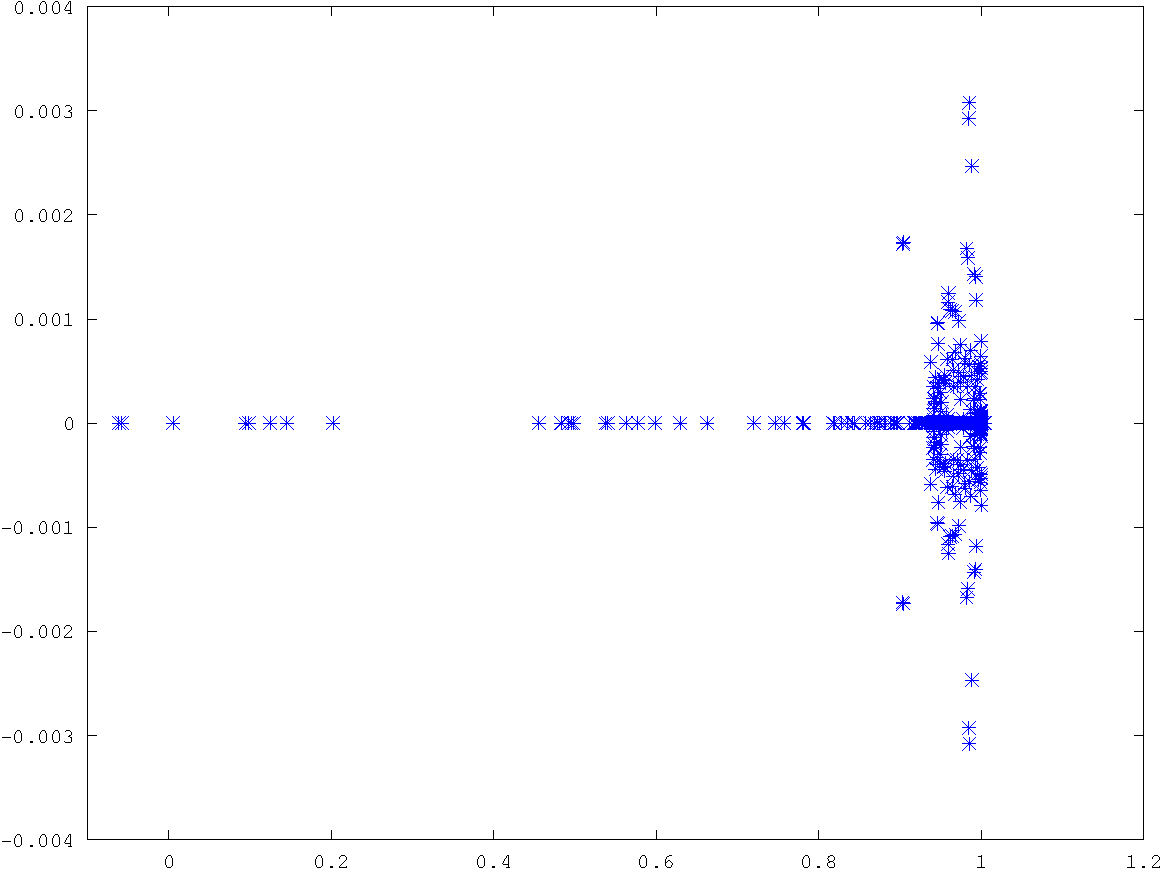
\includegraphics[width=\textwidth]{figures/MG/ElastEigsGMGGalerkinCheb2Unstable.pdf}}
    \end{textblock}
\end{frame}

\begin{frame}[fragile]{Linear solver convergence problems\footnote{\url{http://scicomp.stackexchange.com/questions/513}}}
  \begin{itemize}
  \item Watch the true residual \verb|-ksp_monitor_true_residual|
  \item Make the problem small and create an environment to test rapidly
  \item Are boundary conditions correct? \verb|-pc_type svd -pc_svd_monitor| and \verb|-pc_type lu|
  \item Is the system singular? Known nullspace?
  \item Is the condition number reasonable? \verb|-ksp_monitor_singular_value|
  \item Compare preconditioned residual to true residual (unstable preconditioner)
  \item Is GMRES restart a problem? \verb|-ksp_gmres_restart 300|
  \item Is preconditioner nonlinear? \verb|-ksp_type gcr|, \verb|-ksp_type fgmres|
  \item Geometric multigrid with rediscretization: boundary condition scaling.
  \end{itemize}
\end{frame}
\begin{frame}[fragile]{Nonlinear solver convergence problems\footnote{\url{http://scicomp.stackexchange.com/questions/30}}}
  \begin{itemize}
  \item Is the Jacobian assembled correctly?
    \begin{itemize}
    \item \verb|-snes_mf_operator -pc_type lu|
    \item \verb|-snes_type test| or \verb|-snes_compare_explicit|
    \item \verb|-snes_mf_type ds|
    \end{itemize}
  \item Is the linear system solved accurately enough?
  \item Does the linear system become singular?
  \item Is there a bug in residual evaluation?
  \item Is the residual function discontinuous?
  \item \verb|-snes_linesearch_monitor|
  \item \verb|./configure --with-precision=__float128|
  \end{itemize}
\end{frame}

\section{Coupling approaches}
\begin{frame}{The Great Solver Schism: Monolithic or Split?}
  \begin{columns}
    \begin{column}{0.5\textwidth}
      \begin{block}{Monolithic}
        \begin{itemize}
        \item Direct solvers
        \item Coupled Schwarz
        \item Coupled Neumann-Neumann \\
          (need unassembled matrices)
        \item Coupled multigrid
        \item[X] Need to understand local spectral and compatibility properties of the coupled system
        \end{itemize}
      \end{block}
    \end{column}
    \begin{column}{0.5\textwidth}
      \begin{block}{Split}
        \begin{itemize}
        \item Physics-split Schwarz \\
          (based on relaxation)
        \item Physics-split Schur \\
          (based on factorization)
          \begin{itemize}
          \item  approximate commutators \\
            SIMPLE, PCD, LSC
          \item segregated smoothers
          \item Augmented Lagrangian
          \item ``parabolization'' for stiff waves
          \end{itemize}
        \item[X] Need to understand global coupling strengths
        \end{itemize}
      \end{block}
    \end{column}
  \end{columns}
  \begin{itemize}
  \item Preferred data structures depend on which method is used.
  \item Interplay with geometric multigrid.
  \end{itemize}
\end{frame}

\begin{frame}{Multi-physics coupling in PETSc}
  \begin{columns}
    \begin{column}{0.5\textwidth}
      \tikzstyle{cloud} = [draw, ellipse,fill=red!20, node distance=3cm, minimum height=2em]
      \tikzstyle{block} = [rectangle, draw, fill=blue!20, text width=5em, text centered, rounded corners, minimum height=2em]
      \begin{tikzpicture}
        \node [cloud] (momentum) {Momentum};
        \node [cloud, right of=momentum] (pressure) {Pressure};
        \node<2-> [block, opacity=0.5, fit=(momentum)(pressure), text opacity=0.8] (stokes) {Stokes};
        \node<3-> [cloud, below=2em of momentum] (energy) {Energy};
        \node<3-> [cloud, below=2em of pressure] (geometry) {Geometry};
        \node<4-> [block, opacity=0.4, fit=(stokes)(momentum)(pressure)(energy)(geometry), text opacity=0.8, text height=4em] (ice) {Ice};
        \node<5-> [block, below=2em of ice, minimum width=16em] (bl) {{Boundary \nolinebreak Layer}};
        \node<5-> [block, below=2em of bl, minimum width=16em] (ocean) {Ocean};
        % ]
      \end{tikzpicture}
    \end{column}
    \begin{column}{0.5\textwidth}
      \begin{itemize}
      \item package each ``physics'' independently
      \item solve single-physics and coupled problems
      \item semi-implicit and fully implicit
      \item reuse residual and Jacobian evaluation unmodified
      \item direct solvers, fieldsplit inside multigrid, multigrid inside fieldsplit without recompilation
      \item use the best possible matrix format for each physics \\ (e.g. symmetric block size 3)
      \item matrix-free anywhere
      \item multiple levels of nesting
      \end{itemize}
    \end{column}
  \end{columns}
\end{frame}

\begin{frame}{Splitting for Multiphysics}
  \begin{equation*}
    \begin{bmatrix}
      A & B \\ C & D
    \end{bmatrix}
    \begin{bmatrix}
      x \\ y
    \end{bmatrix}
    =
    \begin{bmatrix}
      f \\ g
    \end{bmatrix}
  \end{equation*}
  \begin{itemize}\item Relaxation:
    \code{-pc\_fieldsplit\_type [additive,multiplicative,symmetric\_multiplicative]}
    \begin{equation*}
      \begin{bmatrix}
        A & \\  & D
      \end{bmatrix}^{-1} \qquad 
      \begin{bmatrix}
        A & \\ C & D
      \end{bmatrix}^{-1} \qquad
      \begin{bmatrix}
        A & \\  & \bm 1
      \end{bmatrix}^{-1}
      \left(
        \bm 1 -
        \begin{bmatrix}
          A & B \\ & \bm 1
        \end{bmatrix}
        \begin{bmatrix}
          A & \\ C & D
        \end{bmatrix}^{-1}
      \right)
    \end{equation*}
    \begin{itemize}
    \item Gauss-Seidel inspired, works when fields are loosely coupled
    \end{itemize}
  \item Factorization: \code{-pc\_fieldsplit\_type schur}
    \begin{align*}
      \begin{bmatrix}
        A & B \\ & S
      \end{bmatrix}^{-1}
      \begin{bmatrix}
        1 & \\ CA^{-1} & 1
      \end{bmatrix}^{-1}, \qquad
      S = D - C A^{-1} B
    \end{align*}
    \begin{itemize}
    \item robust (exact factorization), can often drop lower block
    \item how to precondition $S$ which is usually dense?
      \begin{itemize}
      \item interpret as differential operators, use approximate commutators
      \end{itemize}
    \end{itemize}
  \end{itemize}
\end{frame}

\begin{frame}
  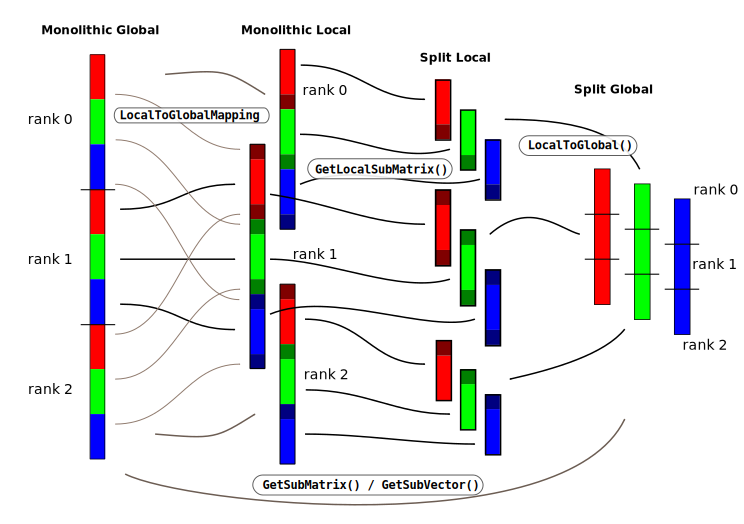
\includegraphics[width=\textwidth]{figures/PETSc/LocalSpaces} \\[-.5em]
  Work in Split Local space, matrix data structures reside in any space.
\end{frame}

\begin{frame}[fragile]{Multiphysics Assembly Code: Jacobians}
\begin{minted}[fontsize=\footnotesize]{c}
FormJacobian_Coupled(SNES snes,Vec X,Mat J,Mat B,...) {
  // Access components as for residuals
  MatGetLocalSubMatrix(B,is[0],is[0],&Buu);
  MatGetLocalSubMatrix(B,is[0],is[1],&Buk);
  MatGetLocalSubMatrix(B,is[1],is[0],&Bku);
  MatGetLocalSubMatrix(B,is[1],is[1],&Bkk);
  FormJacobianLocal_U(user,&infou,u,k,Buu);         // single physics
  FormJacobianLocal_UK(user,&infou,&infok,u,k,Buk); // coupling
  FormJacobianLocal_KU(user,&infou,&infok,u,k,Bku); // coupling
  FormJacobianLocal_K(user,&infok,u,k,Bkk);         // single physics
  MatRestoreLocalSubMatrix(B,is[0],is[0],&Buu);
  // More restores
\end{minted}
\begin{itemize}
\item Assembly code is independent of matrix format
\item Single-physics code is used unmodified for coupled problem
\item No-copy fieldsplit: \verb|-pack_dm_mat_type nest -pc_type fieldsplit|
\item Coupled direct solve: \\
  {\scriptsize \verb|-pack_dm_mat_type aij -pc_type lu -pc_factor_mat_solver_package mumps|}
\end{itemize}
\end{frame}

% \begin{frame}
  \alert{\texttt{MatGetLocalSubMatrix(Mat A,IS rows,IS cols,Mat *B);}}
  \begin{itemize}
  \item Primarily for assembly
    \begin{itemize}
    \item \texttt{B} is not guaranteed to implement \texttt{MatMult}
    \item The communicator for \texttt{B} is not specified, \\
      only safe to use non-collective ops (unless you check)
    \end{itemize}
  \item \texttt{IS} represents an index set, includes a block size and communicator
  \item \texttt{MatSetValuesBlockedLocal()} is implemented
  \item MatNest returns nested submatrix, no-copy
  \item No-copy for Neumann-Neumann formats \\ (unassembled across procs, e.g. BDDC, FETI-DP)
  \item Most other matrices return a lightweight proxy \texttt{Mat}
    \begin{itemize}
    \item \texttt{COMM\_SELF}
    \item Values not copied, does not implement \texttt{MatMult}
    \item Translates indices to the language of the parent matrix
    \item Multiple levels of nesting are flattened
    \end{itemize}
  \end{itemize}
\end{frame}


% \begin{frame}[fragile]{Monolithic nonlinear solvers}
  \begin{block}{Coupled nonlinear multigrid accelerated by NGMRES with multi-stage smoothers}
  \begin{Verbatim}[formatcom=\footnotesize]
    -lidvelocity 200 -grashof 1e4
    -snes_grid_sequence 5 -snes_monitor -snes_view
    -snes_type ngmres
    -npc_snes_type fas
    -npc_snes_max_it 1
    -npc_fas_coarse_snes_type ls
    -npc_fas_coarse_ksp_type preonly
    -npc_fas_snes_type ms
    -npc_fas_snes_ms_type vltp61
    -npc_fas_snes_max_it 1
    -npc_fas_ksp_type preonly
    -npc_fas_pc_type pbjacobi
    -npc_fas_snes_max_it 1
  \end{Verbatim}
  \begin{itemize}
  \item Uses only residuals and point-block diagonal
  \item High arithmetic intensity and parallelism
  \end{itemize}
\end{block}
\end{frame}

% \begin{frame}{Nonlinear solvers in PETSc SNES}
  \begin{description}
  \item[LS, TR] Newton-type with line search and trust region
  \item[NRichardson] Nonlinear Richardson, usually preconditioned
  \item[VIRS, VIRSAUG, and VISS] reduced space and semi-smooth methods for variational inequalities
  \item[QN] Quasi-Newton methods like BFGS
  \item[NGMRES] Nonlinear GMRES
  \item[NCG] Nonlinear Conjugate Gradients
  \item[SORQN] Multiplicative Schwarz quasi-Newton
  \item[GS] Nonlinear Gauss-Seidel/multiplicative Schwarz sweeps
  \item[FAS] Full approximation scheme (nonlinear multigrid)
  \item[MS] Multi-stage smoothers, often used with FAS for hyperbolic problems
  \item[Shell] Your method, often used as a (nonlinear) preconditioner
  \end{description}
\end{frame}


\section{Stokes problems}
\begin{frame}[fragile]{Stokes example}
The common block preconditioners for Stokes require only options:
\begin{columns}
\begin{column}[c]{0.67\textwidth}
\only<1>{\begin{center}\Huge The Stokes System\end{center}}
\begin{itemize}
  \item[]<2-> \code{-pc\_type fieldsplit}
  \item[]<2-> \code{-pc\_field\_split\_type \only<2>{additive}\only<3>{multiplicative}\only<4->{schur}}

  \only<1-7>{
  \medskip

% Change ml to hypre and gamg for some

% Slide to say testing is necessary ()
%   Math should guide testing
%   Ask Mark for references about negative results
%   Gives algorithmic pieces to customize for different problems (No Black Box)

  \item[]<2->
    \only<2>{\code{-fieldsplit\_0\_pc\_type ml}}
    \only<3>{\code{-fieldsplit\_0\_pc\_type hypre}}
    \only<4->{\code{-fieldsplit\_0\_pc\_type gamg}}
  \item[]<2-> \code{-fieldsplit\_0\_ksp\_type preonly}

  \medskip

  \item[]<2-> \only<2-3>{\code{-fieldsplit\_1\_pc\_type jacobi}}  \only<4-6>{\code{-fieldsplit\_1\_pc\_type none}} \only<7>{\code{-fieldsplit\_1\_pc\_type lsc}}
  \item[]<2-> \only<2-3>{\code{-fieldsplit\_1\_ksp\_type preonly}}\only<4->{\code{-fieldsplit\_1\_ksp\_type minres}}
  }
\end{itemize}
\end{column}
%
% TODO: Add citations for each solver choice
\begin{column}[c]{0.33\textwidth}
\only<1-7>{
\Huge
\only<2-7>{\begin{center}PC\end{center}}
\begin{equation*}
\left(
\only<1>{
\begin{matrix}
A & B \\
B^T & 0
\end{matrix}
}
\only<2>{
\begin{matrix}
\hat A & 0 \\
    0  & I
\end{matrix}
}
\only<3>{
\begin{matrix}
\hat A & B \\
    0  & I
\end{matrix}
}
\only<4>{
\begin{matrix}
\hat A & 0 \\
    0  & -\hat S
\end{matrix}
}
\only<5>{
\begin{matrix}
\hat A & 0 \\
  B^T  & \hat S
\end{matrix}
}
\only<6>{
\begin{matrix}
\hat A & B \\
    0  & \hat S
\end{matrix}
}
\only<7>{
\begin{matrix}
\hat A & B \\
    0  & \hat S_{\text{LSC}}
\end{matrix}
}
\right)
\end{equation*}
}
\end{column}
\end{columns}

\medskip

\only<4->{
\hskip1pt\quad\ \ \code{-pc\_fieldsplit\_schur\_factorization\_type \only<4>{diag}\only<5>{lower}\only<6-7>{upper}\only<8>{full}}
}

\only<2-7>{\scriptsize
\begin{itemize}
\item[]
  \only<2>{Cohouet and Chabard, \emph{Some fast 3D finite element solvers for the generalized Stokes problem}, 1988.}
  \only<3>{Elman, \emph{Multigrid and Krylov subspace methods for the discrete Stokes equations}, 1994.}
  \only<4-7>{May and Moresi, \emph{Preconditioned iterative methods for Stokes flow problems arising in computational geodynamics}, 2008.}
\item[]
  \only<4>{Olshanskii, Peters, and Reusken, \emph{Uniform preconditioners for a parameter dependent saddle point problem with application to generalized Stokes interface equations}, 2006.}
  \only<7>{Kay, Loghin and Wathen, \emph{A Preconditioner for the Steady-State N-S Equations}, 2002.}
%  \only<7>{Kay, Loghin and Wathen, \emph{A Preconditioner for the Steady-State Navier--Stokes Equations}, 2002.}
  \only<7>{Elman, Howle, Shadid, Shuttleworth, and Tuminaro, \emph{Block preconditioners based on approximate commutators}, 2006.}
\end{itemize}
}%\medskip

\only<8>{
\Huge
\begin{center}PC\end{center}
\begin{equation*}
\left(
\begin{matrix}
      I        &  0 \\
    B^T A^{-1}  &  I
\end{matrix}
\right) \left(
\begin{matrix}
\hat A & 0 \\
    0  & \hat S
\end{matrix}
\right) \left(
\begin{matrix}
 I & A^{-1} B \\
 0 & I
\end{matrix}
\right)
\end{equation*}
}
\end{frame}
%
\begin{frame}[fragile]{Stokes example}
All block preconditioners can be \textit{embedded} in MG using only options:
\begin{columns}
\begin{column}[c]{0.67\textwidth}
\begin{itemize}\scriptsize
  \item[]<1-> \code{-pc\_type mg -pc\_mg\_levels 5 -pc\_mg\_galerkin}
  \item[]<2-> \code{-mg\_levels\_pc\_type fieldsplit}
  \item[]<2-> \code{-mg\_levels\_pc\_fieldsplit\_type \only<2>{additive}\only<3>{multiplicative}\only<4->{schur}}

  \only<2-7>{
  \medskip
  \item[]<2-> \code{-mg\_levels\_fieldsplit\_0\_pc\_type sor}
  \item[]<2-> \code{-mg\_levels\_fieldsplit\_0\_ksp\_type preonly}

  \medskip

  \item[]<2-> \only<2-3>{\code{-mg\_levels\_fieldsplit\_1\_pc\_type jacobi}}  \only<4-6>{\code{-mg\_levels\_fieldsplit\_1\_pc\_type none}} \only<7>{\code{-mg\_levels\_fieldsplit\_1\_pc\_type lsc}}
  \item[]<2-> \only<2-3>{\code{-mg\_levels\_fieldsplit\_1\_ksp\_type preonly}}\only<4->{\code{-mg\_levels\_fieldsplit\_1\_ksp\_type minres}}
  }
\end{itemize}
\end{column}
%
\begin{column}[c]{0.33\textwidth}
\only<2-7>{
\Huge
\only<2-7>{\begin{center}Smoother PC\end{center}}
\begin{equation*}
\left(
\only<1>{
\begin{matrix}
A & B \\
B^T & 0
\end{matrix}
}
\only<2>{
\begin{matrix}
\hat A & 0 \\
    0  & I
\end{matrix}
}
\only<3>{
\begin{matrix}
\hat A & B \\
    0  & I
\end{matrix}
}
\only<4>{
\begin{matrix}
\hat A & 0 \\
    0  & -\hat S
\end{matrix}
}
\only<5>{
\begin{matrix}
\hat A & 0 \\
  B^T  & \hat S
\end{matrix}
}
\only<6>{
\begin{matrix}
\hat A & B \\
    0  & \hat S
\end{matrix}
}
\only<7>{
\begin{matrix}
\hat A & B \\
    0  & \hat S_{\text{LSC}}
\end{matrix}
}
\right)
\end{equation*}
}
\end{column}
\end{columns}

\medskip

\only<4->{\scriptsize
\hskip1pt\quad\ \ \code{-mg\_levels\_pc\_fieldsplit\_schur\_factorization\_type \only<4>{diag}\only<5>{lower}\only<6-7>{upper}}
}

\only<1>{
\Huge
\begin{center}\Huge System on each Coarse Level\end{center}
\begin{equation*}
R \left(
\begin{matrix}
 A    & B \\
 B^T  & 0
\end{matrix}
\right) P
\end{equation*}
}
\end{frame}

\begin{frame}{Smoothing for saddle point systems}
  \begin{equation*}
  \begin{pmatrix}
    A & B^T \\ B & 0
  \end{pmatrix}
  \begin{pmatrix}
    u \\ p
  \end{pmatrix}
  =
  \begin{pmatrix}
    b \\ 0
  \end{pmatrix}
\end{equation*}
  \begin{itemize}
  \item pressure has no self-coupling
  \item pressure error modes not spectrally separated
  \item approaches
    \begin{itemize}
    \item block smoothers (Vanka)
    \item amplify fine-grid modes (distributive relaxation)
    \item splitting with approximate Schur complement
    \end{itemize}
  \end{itemize}
\end{frame}

\begin{frame}{Vanka block smoothers}
  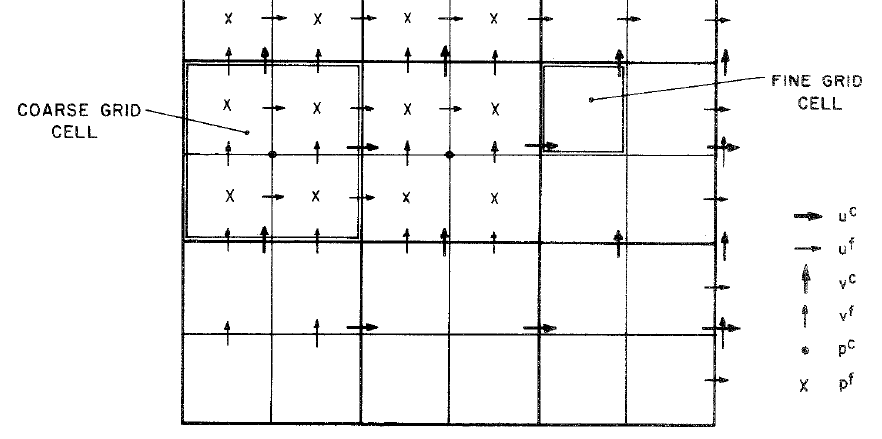
\includegraphics[width=0.9\textwidth]{figures/VankaStaggeredGrid} \\
  \begin{itemize}
  \item solve pressure-centered cell problems \\
    \quad (better for discontinuous pressure)
  \item robust convergence factor $\sim 0.3$ \emph{if} coarse grids are accurate
  \item 1D energy minimizing interpolants easy and effective
  \item can use assembled sparse matrices, but more efficient without
  \end{itemize}
\end{frame}

\begin{frame}{Changing Associativity: Distributive Smoothing}
  \begin{align*}
    P A x &= P b & AP y = b, & \quad x = Py
  \end{align*}
  \begin{itemize}
  \item Normal Preconditioning: make $PA$ or $AP$ well-conditioned
  \item Alternative: amplify high-frequency modes
    \begin{itemize}
    \item Multigrid smoothers only need to relax high-frequency modes
    \item Easier to do when spectrally separated: $h$-ellipticity
      \begin{itemize}
      \item pointwise smoothers (Gauss-Seidel) and polynomial/multistage methods
      \end{itemize}
    \item Mechanics: form the product $PA$ or $AP$ and apply ``normal'' method
    \item Example (Stokes)
      \begin{align*}
        A &\sim \begin{pmatrix} -\nabla^2 & -\nabla \\ \nabla\cdot &
          0 \end{pmatrix} &
        P &\sim \begin{pmatrix} \bm 1 & -\nabla \\ 0 & -\nabla^2 \end{pmatrix} &
        AP &\sim
        \begin{pmatrix}
          -\nabla^2 & \text{``0''} \\ \nabla\cdot & -\nabla^2
        \end{pmatrix}
      \end{align*}
    \end{itemize}
  \end{itemize}
\end{frame}

\begin{frame}[fragile]{Coupled MG for Stokes, split smoothers}
\begin{columns}
  \begin{column}{0.3\textwidth}
    \begin{align*}
      J &=
      \begin{pmatrix}
        A & B^T \\ B & C
      \end{pmatrix} \\
      P_{\text{smooth}} &=
      \begin{pmatrix}
        A_{\text{SOR}} & 0 \\
        B & M
      \end{pmatrix}
    \end{align*}
  \end{column}
  \begin{column}{0.7\textwidth}
    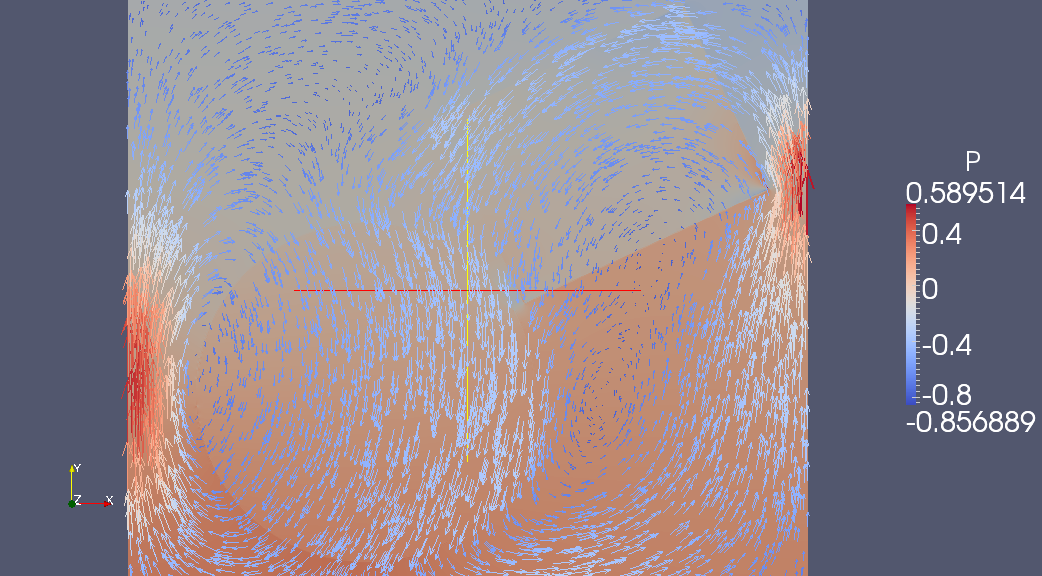
\includegraphics[width=\textwidth]{figures/Sinker2}
  \end{column}
\end{columns}
\begin{Verbatim}[formatcom=\footnotesize]
-pc_type mg -pc_mg_levels 5 -pc_mg_galerkin
-mg_levels_pc_type fieldsplit
-mg_levels_pc_fieldsplit_block_size 3
-mg_levels_pc_fieldsplit_0_fields 0,1
-mg_levels_pc_fieldsplit_1_fields 2
-mg_levels_fieldsplit_0_pc_type sor
\end{Verbatim}
\end{frame}


\section{Performance considerations}
\begin{frame}{Profiling basics}
  \begin{itemize}
  \item Get the math right
    \begin{itemize}
    \item Choose an algorithm that gives robust iteration counts and really converges
    \end{itemize}
  \item Look at where the time is spent
    \begin{itemize}
    \item Run with \texttt{-log\_summary} and look at events
    \item \texttt{VecNorm,VecDot} measures latency
    \item \texttt{MatMult} measures neighbor exchange and memory bandwidth
    \item \texttt{PCSetUp} factorization, aggregation, matrix-matrix products, \ldots
    \item \texttt{PCApply} V-cycles, triangular solves, \ldots
    \item \texttt{KSPSolve} linear solve
    \item \texttt{SNESFunctionEval} residual evaluation (user code)
    \item \texttt{SNESJacobianEval} matrix assembly (user code)
    \end{itemize}
  \end{itemize}
\end{frame}
\begin{frame}[shrink=5]{Performance of assembled versus unassembled}
  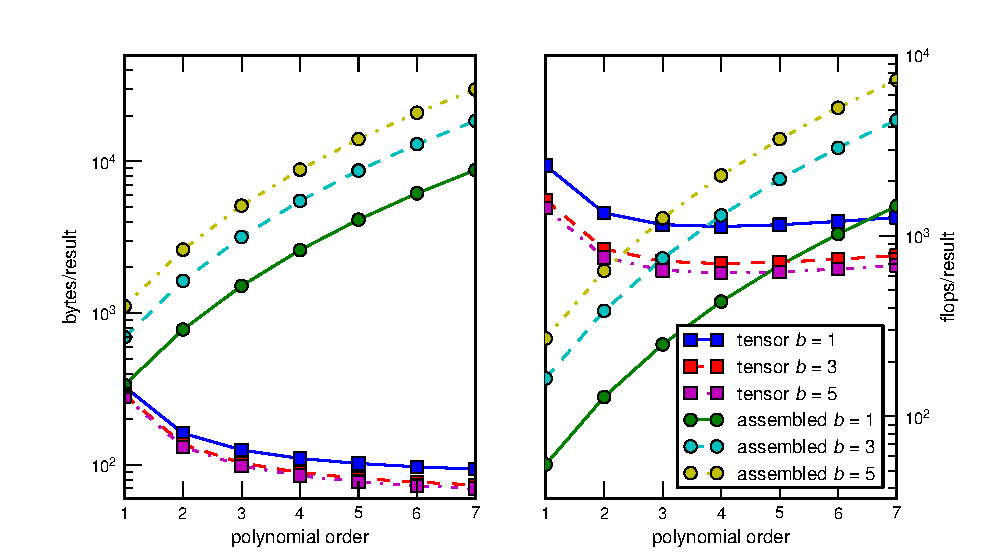
\includegraphics[width=\textwidth]{figures/TensorVsAssembly} \\
  \begin{itemize}
  \item High order Jacobian stored unassembled using coefficients at quadrature points, can use local AD
  \item Choose approximation order at run-time, independent for each field
  \item Precondition high order using assembled lowest order method
  \item Implementation $> 70\%$ of FPU peak, SpMV bandwidth wall $< 4\%$
  \end{itemize}
\end{frame}

\begin{frame}{Hardware Arithmetic Intensity}
  \begin{tabular}{lc}
    \toprule
    Operation                         & Arithmetic Intensity (flops per byte) \\
    \midrule
    Sparse matrix-vector product      & 1/6                  \\
    Dense matrix-vector product       & 1/4                  \\
    Unassembled matrix-vector product & $\approx 8$          \\
    High-order residual evaluation    & $> 5$                \\
    \bottomrule
  \end{tabular}
  \bigskip
  \begin{tabular}{lrrr}
    \toprule
    Processor           & BW (GB/s) & Peak (GF/s) & Balanced AI (F/B) \\
    \midrule
    Sandy Bridge 6-core & 21*       & 150         & 7.2                 \\
    Magny Cours 16-core & 42*       & 281         & 6.7                 \\
    Blue Gene/Q node    & 43        & 205         & 4.8                 \\
    GeForce 9400M       & 21        & 54          & 2.6                 \\
    GTX 285             & 159       & 1062        & 6.8                 \\
    Tesla M2050         & 144       & 1030        & 7.1                 \\
    \bottomrule
  \end{tabular}
\end{frame}

\begin{frame}[shrink=5]{Quasi-Newton revisited: ameliorating setup costs}
  \begin{textblock}{0.25}[1,0](0.99,0.2)
    {\small pseudo-plastic rheology} \\
    {\scriptsize
      \texttt{-snes\_type qn
        -snes\_qn\_scale\_type jacobian}}
  \end{textblock}

    \begin{itemize}
    \item Newton-Krylov with analytic Jacobian
{\footnotesize
      \begin{tabular}{lllll}
        \toprule
        Lag & FunctionEval & JacobianEval & PCSetUp & PCApply \\
        \midrule
        % 14 & 11 & 11 & 11 \\
        1 bt & 12 & 8 & 8 & 31 \\
        1 cp & 31 & 6 & 6 & 24 \\
        2 bt & \multicolumn{4}{c}{--- diverged ---} \\
        2 cp & 41 & 4 & 4 & 35 \\
        3 cp & 50 & 4 & 4 & 44 \\
        \bottomrule
      \end{tabular}
}
    \item Jacobian-free Newton-Krylov with lagged preconditioner
{\footnotesize
      \begin{tabular}{lllll}
        \toprule
        Lag & FunctionEval & JacobianEval & PCSetUp & PCApply \\
        \midrule
        1 bt & 23 & 11 & 11 & 31 \\
        2 bt & 48 & 4 & 4 & 36 \\
        3 bt & 64 & 3 & 3 & 52 \\
        4 bt & 87 & 3 & 3 & 75 \\
        \bottomrule
      \end{tabular}
}
    \item Limited-memory Quasi-Newton/BFGS with lagged solve for $H_0$
{\footnotesize
      \begin{tabular}{llllll}
        \toprule
        Restart & $H_0$ & FunctionEval & JacobianEval & PCSetUp & PCApply \\
        \midrule
        1 cp & $10^{-5}$ & 17 & 4 & 4 & 35 \\
        1 cp & preonly & 21 & 5 & 5 & 10 \\
        3 cp & $10^{-5}$ & 21 & 3 & 3 & 43 \\
        3 cp & preonly & 23 & 3 & 3 & 11 \\
        6 cp & $10^{-5}$ & 29 & 2 & 2 & 60 \\
        6 cp & preonly & 29 & 2 & 2 & 14 \\
        \bottomrule
      \end{tabular}
}
    \end{itemize}
\end{frame}

\begin{frame}{Network latency}
  \begin{block}{\texttt{MPI\_Allreduce} is slow at large scale}
    \begin{itemize}
    \item True on many machines, not on Blue Gene ($\sim \SI{100}{\micro\second}$)
    \item Bottleneck for Krylov methods
    \item Pipelining allows overlap, uses \texttt{MPI\_Iallreduce} from MPI-3\\
      \texttt{-ksp\_type pgmres}, \texttt{-ksp\_type pipecg}, \texttt{-ksp\_type pipecr}
    \end{itemize}
  \end{block}
  \begin{block}{Coarse grid solves for multigrid}
    \begin{itemize}
    \item Need to restrict active processor set
    \item Coarse levels have similar cost to finer levels
    \item Aggressive coarsening more important than tight iteration count
    \item Additive multigrid possible, but less robust
    \end{itemize}
  \end{block}
\end{frame}

\begin{frame}{Outlook}
  \begin{itemize}
  \item PETSc \url{http://mcs.anl.gov/petsc}
  \item Trilinos \url{http://trilinos.sandia.gov}
  \item Think about solution algorithms when designing discretization
  \item Learn how to evaluate solver quality and experiment
  \item Expect the best method to change with problem instance and machine
  \end{itemize}
  \begin{block}{Contact}
    \begin{itemize}
    \item \url{petsc-maint@mcs.anl.gov}
    \item \url{http://lists.mcs.anl.gov/pipermail/petsc-users/}
    \item \url{http://scicomp.stackexchange.com}
    \end{itemize}
  \end{block}
\end{frame}

\end{document}
